\chapter{評価}
\label{chap:evaluation}

本章では、本論文で実装した通知システムの評価を行う。そのために、まずはインスリン摂取検知デバイスと食事検知デバイスを個別に評価する。
そして、最後に2つを組み合わせて全体の通知システムを評価し、結果を受けて、本提案手法が本論文であげた解決したい問題を解決できるものであるか考察していく。

\section{インスリン摂取検知デバイス}
本節では、インスリン注射器に見立てたペンに装着されたインスリン摂取検知デバイスの評価を行う。

\subsection{評価方法}
第\ref{chap:diabetes}章でも述べた通り、糖尿病患者のインスリン治療では、ペン型のインスリン注射器を用いて必要な量のインスリンを服用する。
そして、本論文の評価では、この動作が再現でき、その動作を以ってインスリン摂取とすれば良い。
よって、今回はインスリンを実際に摂取するのではなく擬似的に\textbf{ペンを握り、5秒間スイッチを押して静止する}\cite{how_to_inject_insulin_1}\cite{how_to_inject_insulin_2}
という動作を行うことでインスリン摂取を行ったとみなした。
今回は、これを10回試行し、試行間隔は約10秒で行い、Webサーバーを通してその時間が正確に記録されているかどうかを確認した。
試行間隔は10秒、そして検知のための静止時間は5秒であるため、検知時間の間隔は約15秒になっていることが期待される。

\subsection{結果}

表\ref{tb:insulin_detection_time}が、インスリン摂取検知デバイスを使用して上記の動作を10回試行した結果である。
\textbf{\textit{injected\_time}}が、インスリン摂取検知デバイスから送られた検知時間であり、\textbf{\textit{created\_at}}がMySQLに保存された時間である。
この結果から、検知された時間が正確かつ即時的に保存されていることがわかる。

\newpage

\begin{table}[htbp]
  \caption{インスリン摂取検知デバイスによってリクエストされ、保存されたデータ}
  \label{tb:insulin_detection_time}
  \begin{center}
    \begin{tabular}{|c||l|l|}
      \hline
      ID & injected\_time & created\_at \\\hline
      1 & 2021-01-24 00:24:58 & 2021-01-24 00:24:58 \\\hline
      2 & 2021-01-24 00:25:13 & 2021-01-24 00:25:13 \\\hline
      3 & 2021-01-24 00:25:28 & 2021-01-24 00:25:28 \\\hline
      4 & 2021-01-24 00:25:44 & 2021-01-24 00:25:44 \\\hline
      5 & 2021-01-24 00:25:59 & 2021-01-24 00:25:59 \\\hline
      6 & 2021-01-24 00:26:13 & 2021-01-24 00:26:13 \\\hline
      7 & 2021-01-24 00:26:28 & 2021-01-24 00:26:29 \\\hline
      8 & 2021-01-24 00:26:44 & 2021-01-24 00:26:44 \\\hline
      9 & 2021-01-24 00:27:00 & 2021-01-24 00:27:00 \\\hline
      10 & 2021-01-24 00:27:15 & 2021-01-24 00:27:15 \\\hline
    \end{tabular}
  \end{center}
\end{table}

\subsection{考察}

結果から、10回全て約15秒間隔でインスリン摂取検知時間が取得できており、インスリン摂取検知デバイスは期待した通り動作していることが確認できた。

\section{食事検知デバイス}
\label{section:meal_detect_eval}

本節では、食事検知デバイスの評価を行う。

\subsection{評価手法}
作成した食事検知デバイスを食卓上に置き、場面別で様々な動作を行い、食事の場面では\textbf{食事として検知}、それ以外の場合は\textbf{食事ではない}として、検知しないことを期待する。

今回評価を行った卓上での行動は以下の通りである。

\begin{enumerate}
  \item 食事をする
  \item パソコンで作業する
  \item ものを書く
  \item 机を拭く
\end{enumerate}

1の\textbf{食事をする}では、図\ref{fig:experiment_food1}のような1主3菜のメニュー、図\ref{fig:experiment_food2}のようなパスタのみの食事、図\ref{fig:experiment_food3}のような丼、
図\ref{fig:experiment_food4}のようなフォークナイフを使うステーキメニューを被験者に食べてもらった。図\ref{fig:experiment}が実際の実験の様子である。
2の\textbf{パソコンで作業する}では、タイピングが机に与える主な振動となるため、寿司打\cite{sushida}やメッセージのやりとりなどを10分間行ってもらった。
3の\textbf{ものを書く}では、ペンで何かを書く動作、消しゴムで消す動作、消しカスを払う動作、の3つが主な振動源となるためその3つを満たせるよう数学の問題を解く、絵を描くなどを行ってもらった。
4の\textbf{机を拭く}では、ペーパータオルで机を拭いてもらった。

さらに追加評価で以下のものを行なってもらった

\begin{enumerate}
  \item お茶を飲む
  \item マウスを使ってネットサーフィン
\end{enumerate}

追加評価における、
1の\textbf{お茶を飲む}では、
2の\textbf{マウスを使ってネットサーフィン}では、文字通りマウスを使ったポインターの移動とタイピングをしながらネットサーフィンを行なってもらった。

これらの動作の際に起こる振動に対しても食事検知デバイスで正確に食事のみ検知できるかを評価する。

\begin{figure}[htbp]
  \caption{今回評価の際に食べてもらった1主3菜の一例}
  \label{fig:experiment_food1}
  \begin{center}
    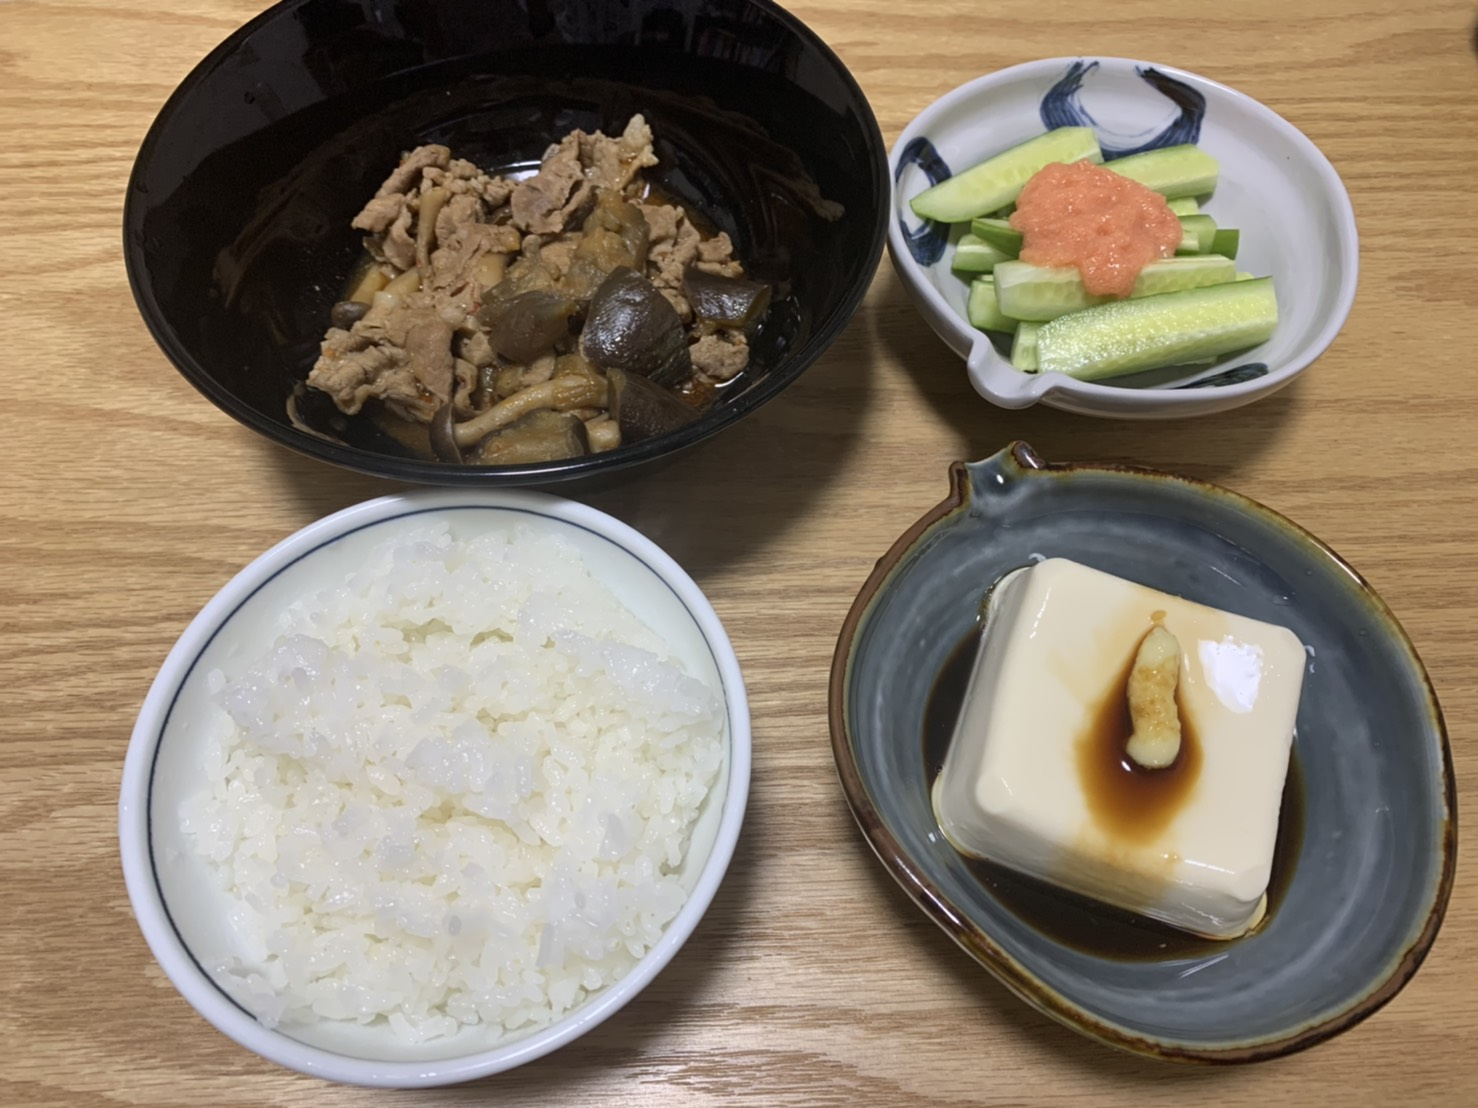
\includegraphics[bb=0 0 1450 1200,width=15cm]{assets/experiment_food1.jpg}
  \end{center}
\end{figure}

\begin{figure}[htbp]
  \caption{今回評価の際に食べてもらったパスタの一例}
  \label{fig:experiment_food2}
  \begin{center}
    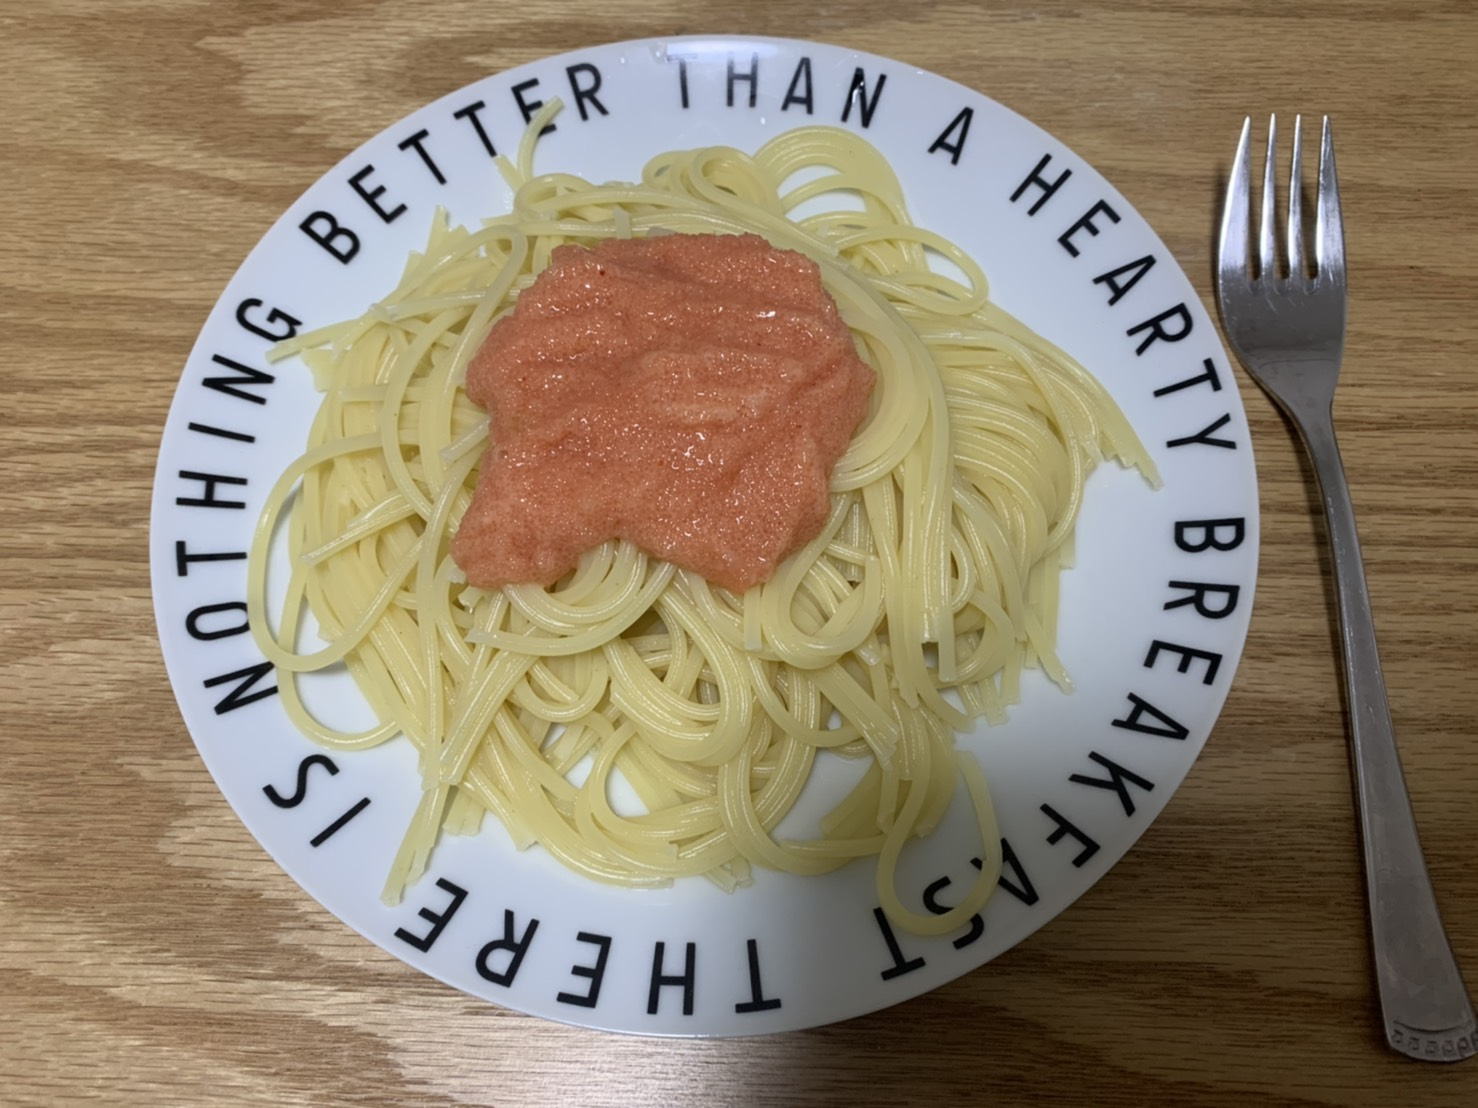
\includegraphics[bb=0 0 1450 1200,width=15cm]{assets/experiment_food2.jpg}
  \end{center}
\end{figure}

\begin{figure}[htbp]
  \caption{今回評価の際に食べてもらった丼の一例}
  \label{fig:experiment_food3}
  \begin{center}
    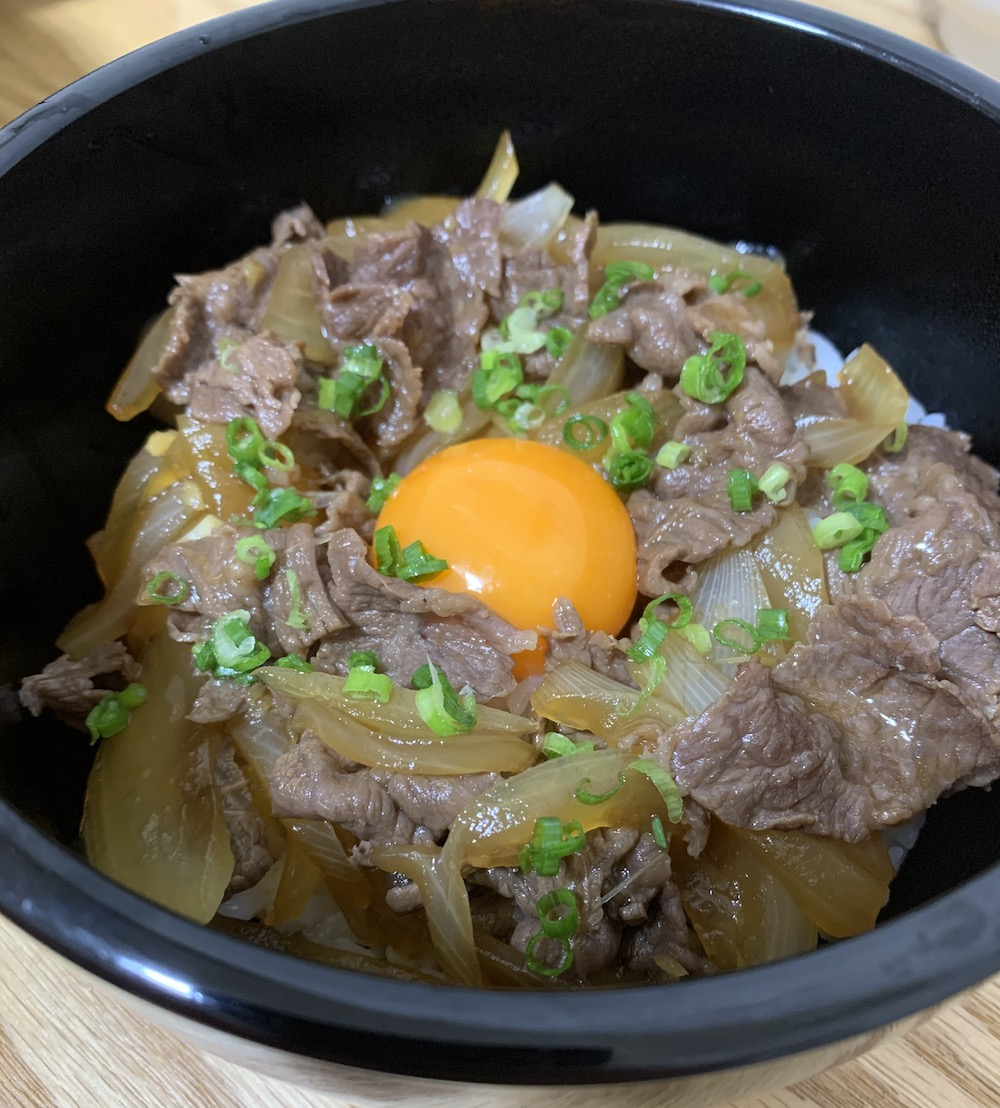
\includegraphics[bb=0 0 1000 1200,width=10cm]{assets/experiment_food3.jpg}
  \end{center}
\end{figure}

\begin{figure}[htbp]
  \caption{今回評価の際に食べてもらったステーキの一例}
  \label{fig:experiment_food4}
  \begin{center}
    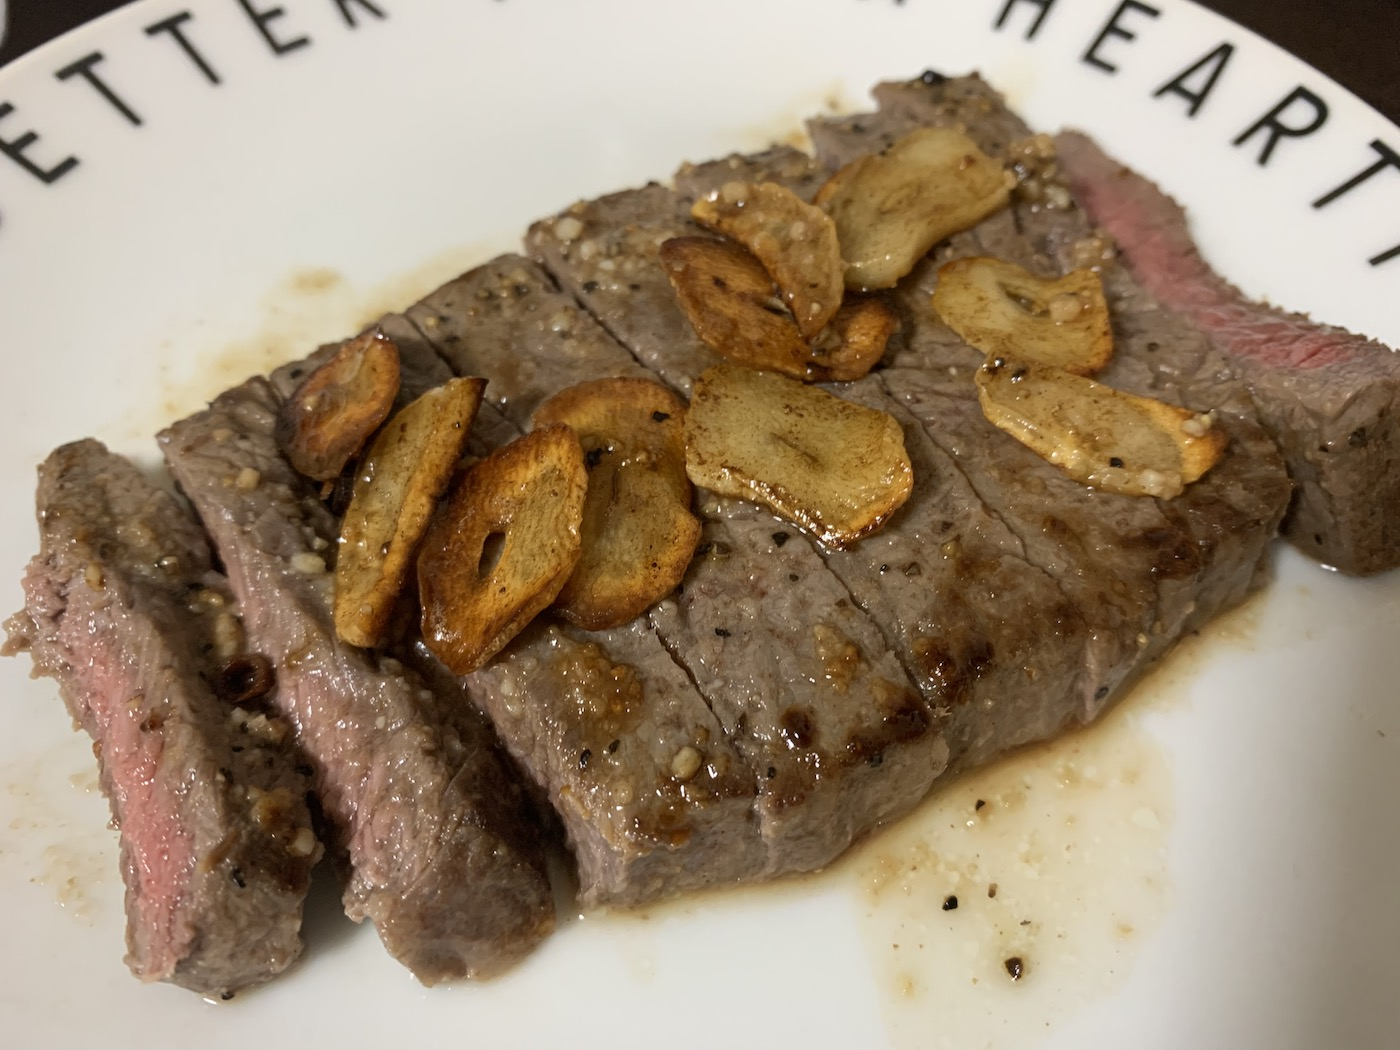
\includegraphics[bb=0 0 1450 1200,width=15cm]{assets/experiment_food4.jpg}
  \end{center}
\end{figure}

\begin{figure}[htbp]
  \caption{実験の様子}
  \label{fig:experiment}
  \begin{center}
    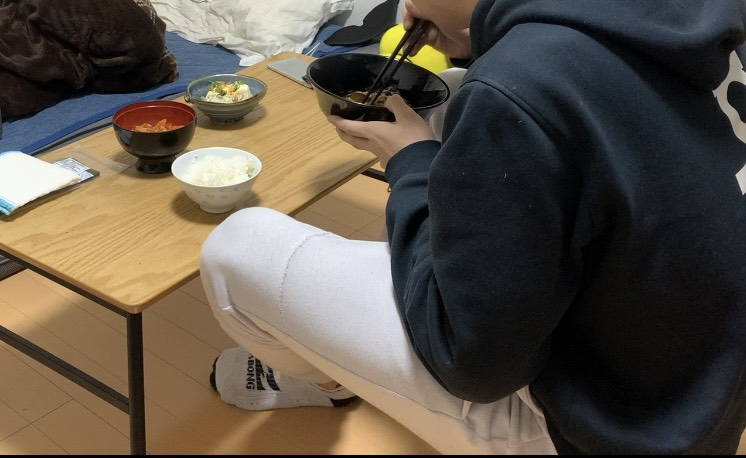
\includegraphics[bb=0 0 700 500,width=15cm]{assets/experiment.jpg}
  \end{center}
\end{figure}

\subsection{結果}

本論文の評価では、20代男性3人、20代女性1人、合計4人の被験者で、食事の検知実験とその他の動作の検知実験を行った。
表\ref{tb:meal_detection_result}が、それぞれの実験の正解検知率である。

% \begin{table}[htbp]
%   \caption{それぞれの被験者の食事時間と食事検知時間}
%   \label{tb:meal_detection_result}
%   \begin{center}
%     \begin{tabular}{|c||c|c|}
%       \hline
%       被験者  & 食事時間 & 食事検知時間 \\
%       \hline\hline
%       被験者A & 2021-01-24 18:53:35 - 19:01:12 & 2021-01-24 18:55:28.264315 \\\hline
%       被験者B & 2021-01-24 19:04:05 - 19:11:10 & 2021-01-24 19:04:28.447520 \\\hline
%       被験者C & 2021-01-21 12:46:51 - 12:58:30 & 2021-01-21 12:49:10.842095 \\\hline
%     \end{tabular}
%   \end{center}
% \end{table}

\begin{table}[htbp]
  \caption{箸で行った正解検知率(nは試行回数)}
  \label{tb:others_detection_result}
  \begin{center}
    \begin{tabular}{|c||c|c|}
      \hline
       & 正解検知率 & 無検知時の平均カウント \\
      \hline\hline
      被験者A (n=1) & 100\% & なし \\\hline
      被験者B (n=1) & 0\% & 3.40 \\\hline
      被験者C (n=24) & 72.00\% & 3.43 \\\hline
      被験者D (n=24) & 84.00\% & 3.50 \\\hline
    \end{tabular}
  \end{center}
\end{table}

今回は、食事以外の動作で検知しなかったことを\textbf{正解}とし、検知してしまった場合には\textbf{不正解}として記述する。
表\ref{tb:others_detection_percentage}が、その他の、パソコンでの作業、ものを書く、机を拭く動作をした時の正解率であり、
表\ref{tb:others_detection_count}が無検知(正解)だった時にの最大カウントの平均を示した。

\begin{table}[htbp]
  \caption{それぞれの被験者がその他の動作を行った時の正解率(nは試行回数)}
  \label{tb:others_detection_percentage}
  \begin{center}
    \begin{tabular}{|c||c|c|c|}
      \hline
       & パソコンでの作業 & 書き物 & 机を拭く \\
      \hline\hline
      被験者A  & 100\% (n=2) & 100\% (n=2) & 100\% (n=2) \\\hline
      被験者B  & 100\% (n=2) & 50\% (n=2) & 100\% (n=2) \\\hline
      被験者C & 100\% (n=10) & 100\% (n=5) & 100\% (n=10) \\\hline
      被験者D & 100\% (n=10) & 100\% (n=5) & 100\% (n=10) \\\hline
    \end{tabular}
  \end{center}
\end{table}

\begin{table}[htbp]
  \caption{それぞれの被験者がその他の動作を行った際に無検知(正解)だった時の平均カウント数(nは無検知回数)}
  \label{tb:others_detection_count}
  \begin{center}
    \begin{tabular}{|c||c|c|c|}
      \hline
       & パソコンでの作業 & 書き物 & 机を拭く \\
      \hline\hline
      被験者A  & 0.50 (n=2) & 1.00 (n=2) & 1.00 (n=2) \\\hline
      被験者B  & 3.00 (n=2) & 1.00 (n=1) & 1.70 (n=2) \\\hline
      被験者C & 0.90 (n=10) & 1.00 (n=5) & 2.00 (n=10) \\\hline
      被験者D & 1.10 (n=10) & 1.20 (n=5) & 1.89 (n=10) \\\hline
    \end{tabular}
  \end{center}
\end{table}

表\ref{tb:others_detection_time}が、その他の、パソコンでの作業、ものを書く、机を拭く動作をしてもらった時間であり、
表\ref{tb:others_detection_result}その食事検知デバイスの検知結果である。

\begin{table}[htbp]
  \caption{追加評価の正解率(nは試行回数)}
  \label{tb:additional_detection_percentage}
  \begin{center}
    \begin{tabular}{|c||c|c|c|}
      \hline
       & お茶を飲む  & マウスを使ってネットサーフィン \\
      \hline\hline
      被験者C & 80\% (n=5) & 80\% (n=5) \\\hline
      被験者D & 80\% (n=5) & 100\% (n=5) \\\hline
    \end{tabular}
  \end{center}
\end{table}


\begin{table}[htbp]
  \caption{追加評価の無検知(正解)だった時の最大カウント数の平均(nは無検知回数)}
  \label{tb:additional_detection_count}
  \begin{center}
    \begin{tabular}{|c||c|c|c|}
      \hline
       & お茶を飲む  & マウスを使ってネットサーフィン \\
      \hline\hline
      被験者C & 2.75 (n=4) & 1.20 (n=4) \\\hline
      被験者D & 2.00  (n=4) & 1.00 (n=5) \\\hline
    \end{tabular}
  \end{center}
\end{table}

% \begin{table}[htbp]
%   \caption{それぞれの被験者がその他の動作を行った時間}
%   \label{tb:others_detection_time}
%   \begin{center}
%     \begin{tabular}{|c||c|c|c|}
%       \hline
%        & パソコンでの作業 & 書き物 & 机を拭く \\
%       \hline\hline
%       被験者A & 2021-01-24 19:39 - 19:47 & 2021-01-24 19:59 - 20:13 & 2021-01-24 20:31 - 20:32 \\\hline
%       被験者B & 2021-01-24 19:50 - 19:57 & 2021-01-24 20:23 - 20:29 & 2021-01-24 20:38 - 20:38  \\\hline
%       被験者C & 2021-01-26 16:36 - 16:43 & 2021-01-26 16:44 - 16:52 & 2021-01-26 16:53 - 16:53 \\\hline
%     \end{tabular}
%   \end{center}
% \end{table}

% \begin{table}[htbp]
%   \caption{それぞれの被験者がその他の動作を行った時の検知結果}
%   \label{tb:others_detection_result}
%   \begin{center}
%     \begin{tabular}{|c||c|c|c|}
%       \hline
%        & パソコンでの作業 & 書き物 & 机を拭く \\
%       \hline\hline
%       被験者A & 検知なし & 検知なし & 検知なし \\\hline
%       被験者B & 検知なし & 検知なし & 検知なし \\\hline
%       被験者C & 検知なし & 検知なし & 検知なし \\\hline
%     \end{tabular}
%   \end{center}
% \end{table}

\subsection{考察}

食事の検知に関して、複数皿があり、箸を主に使用する食事においては、皿の持ち上げが起こりやすく、机に食器を置く機会が多いため、食事検知に至った。しかしながら、
パスタやステーキといった、食器を持ち上げることなく食事ができてしまうものでは、机への振動が弱く、食事として検知するには至らないこともあった。パスタを食事した際に検知したケースは、
具材をフォークで混ぜる際に皿に伝わった振動によるものであった。

また、その他の動作で誤検知が行われたのは、書き物、お茶を飲む行為、そしてマウスを使ってのネットサーフィンであった。書き物に関しては、ノートや書物を置く時の振動、
書く時に腕を置き直すような時の振動が主な振動源となっておりこれを連続で検知したことが誤検知に至った原因であった。お茶を飲む行為の際は、お茶が熱い状態で、
複数回に分けて飲む必要がある場面、そしてそれを急いで飲むような場合に誤検知となったが、すぐに飲める温度の場合には2分以内に6度もコップを置くことなく飲み干してしまうか、
2分以内に定期的には飲まないことがほとんどであった。
マウスを使ってのネットサーフィンでは、ポインターを移動する際にマウスを空中に持って、置く動作を繰り返しながら動かした場合は検知が行われたが、机に付けたまま動かして操作した場合には検知されなかった。

食事場面における食事検知の総正解検知率は64\%となった。被験者AとBに関して、試行回数が1回になってしまったため正確な検知率が出なかったが、被験者CとDの平均では78.00\%と、高い精度で検知できたことになる。
今回の評価により、限定的ではあるが、ある特定の食事に関しては食事を検知することは可能であることを示す結果となった。

\section{インスリン摂取忘れ通知}
ここまでで評価した2つのモジュールを使用して、最終的にインスリン摂取を忘れている際に通知が行えるかどうかを評価する。
本節では、食事検知デバイスの評価の際に参加してもらった20代女性に再度協力してもらい、評価を行った。

\subsection{評価手法}

本評価では、シナリオを2つ用意し、それぞれの期待する結果が得られるかどうかを評価した。
被験者は、本章第\ref{section:meal_detect_eval}節で示したような食事内容で3回ずつシナリオに従って実験を行った。

\subsubsection{シナリオ}

本研究では、以下の2つを実験シナリオとして実施した。

\begin{enumerate}
  \item
    \begin{description}
      \item[インスリン摂取後に食事]\mbox{}\\
        被験者は、インスリン摂取検知デバイスを使用して、食前にインスリン投与と同じアクション(インスリン摂取検知デバイスのスイッチを押して5秒静止)を行う。
        投与のアクションを終えたのち、食事を開始する。
    \end{description}
  \begin{description}
    \item[期待する結果]\mbox{}\\
      インスリン注射器に装着されたデバイスが送信した投与時間は食事検知時間よりも前で、インスリンが正常に投与されたものとして判定。アラートの音声は発されない。
  \end{description}
  \item
    \begin{description}
      \item[インスリン摂取なしで食事]\mbox{}\\
        被験者は、インスリン検知デバイスを使用することなく、食事を始める。
    \end{description}
    \begin{description}
      \item[期待する結果]\mbox{}\\
        食事検知時に直近30分で、インスリンが正常に投与されなかったものとして判定。アラートの音声が発される。
    \end{description}
\end{enumerate}

\subsection{結果}
表\ref{tb:result_scenarios}が、評価結果である。
期待した通りの結果が得られたことを\textbf{正解}、そうでなかった場合に\textbf{不正解}として記述した。
期待した通り、シナリオ1では、食事検知が行われたものの、インスリンが食事前に摂取されていたため、通知は行われなかった。
そしてシナリオ2では、食事検知が行われ、食事前のインスリン摂取が行われていなかったため、期待した通り通知が行われた。

\begin{table}[htbp]
  \caption{シナリオ別の正解率}
  \label{tb:result_scenarios}
  \begin{center}
    \begin{tabular}{|c||c|}
      \hline
      シナリオ No.  & 結果 \\
      \hline\hline
      1  & 通知なし 100\% (n=3) \\\hline
      2 & 通知あり 66.67\% (食事が検知された際の通知率は100\%) (n=3) \\\hline
    \end{tabular}
  \end{center}
\end{table}

% \begin{table}[htbp]
%   \caption{シナリオ1のインスリン摂取時間}
%   \label{tb:scenario_1_insulin}
%   \begin{center}
%     \begin{tabular}{|c||c|c|}
%       \hline
%       ID  & injected\_time & created\_at \\
%       \hline\hline
%       1 &  &  \\\hline
%       2 &  &  \\\hline
%     \end{tabular}
%   \end{center}
% \end{table}

% \begin{table}[htbp]
%   \caption{シナリオ1の食事時間}
%   \label{tb:scenario_2_meal}
%   \begin{center}
%     \begin{tabular}{|c||c|}
%       \hline
%         & 食事時間 \\
%       \hline\hline
%       被験者C & \\\hline
%     \end{tabular}
%   \end{center}
% \end{table}

% \begin{table}[htbp]
%   \caption{シナリオ1の食事検知時間}
%   \label{tb:scenario_1_meal}
%   \begin{center}
%     \begin{tabular}{|c|}
%       \hline
%       検知時間 \\
%       \hline\hline
%        \\\hline
%     \end{tabular}
%   \end{center}
% \end{table}

% \begin{table}[htbp]
%   \caption{シナリオ2の食事時間}
%   \label{tb:scenario_2_meal}
%   \begin{center}
%     \begin{tabular}{|c|}
%       \hline
%        食事時間 \\
%       \hline\hline
%       2021-01-26 20:45:45 - 21:06:12 \\\hline
%        \\\hline
%        \\\hline
%     \end{tabular}
%   \end{center}
% \end{table}

% \begin{table}[htbp]
%   \caption{シナリオ2の食事検知時間}
%   \label{tb:scenario_2_meal_detect}
%   \begin{center}
%     \begin{tabular}{|c|}
%       \hline
%       検知時間 \\
%       \hline\hline
%       2021-01-26 20:48:02.713074 \\\hline
%     \end{tabular}
%   \end{center}
% \end{table}

\subsection{考察}

以上の結果から、知をすべきでないシナリオ1では通知は行われなかったが、これに関しては、食事の検知の有無は関係なく、結果が100\%となった。
しかしながら、シナリオ2に関しては、試行した3回のうち、3回目の試行で食事が検知されず、通知が行われなかった。
その際の食事では食器が卓上にゆっくりと置かれており、それによる振動の大きさが小さかったことが原因と考えられる。
食事検知が正確に行われる限りにおいては100\%通知が行われていたため、食事検知から通知の流れの実装部分は保証されたが、
この提案手法はやはり食事検知の精度に大きくよるものであり、食器の置き方、食事内容などの他の要因によって左右されてしまうことがわかった。

